\documentclass[fleqn]{beamer}

\usepackage{amsmath}
\usepackage{animate}
\usepackage{amsfonts}
\usepackage[mathscr]{eucal}
\usepackage{subcaption}
\usepackage{wrapfig}
\usepackage{graphicx}

\usepackage{fancyhdr}
\usepackage{pstricks}
\usepackage{pst-func}
\usepackage{pst-plot}
\usepackage[utf8x]{inputenc}
\usepackage[spanish]{babel}


\setbeamertemplate{navigation symbols}{}
\definecolor{UniBlue}{RGB}{83,121,170}
\setbeamercolor{frametitle}{fg=black,bg=white}
\setbeamercolor{title}{fg=black,bg=yellow!85!orange}
%\setbeamercolor{title}{fg=red,bg=yellow!90!blue}
\usetheme{Madrid}

\beamersetuncovermixins{\opaqueness<1>{25}}{\opaqueness<2->{15}}
\begin{document}

\title{Laboratorio de CGeIHC}
\author{Reynaldo Martell}
\date{\today} 

\begin{frame}
\titlepage
\end{frame}

\begin{frame}\frametitle{\rule{0mm}{10mm}\rule{5mm}{0mm} Laboratorio de CGeIHC. }
Laboratorio de Proyectos Externos 2, Planta Baja, Edificio U - "Bernardo
Quintana Arrioja“, Facultad de Ingeniería
\begin{figure}[H]
	\centering
	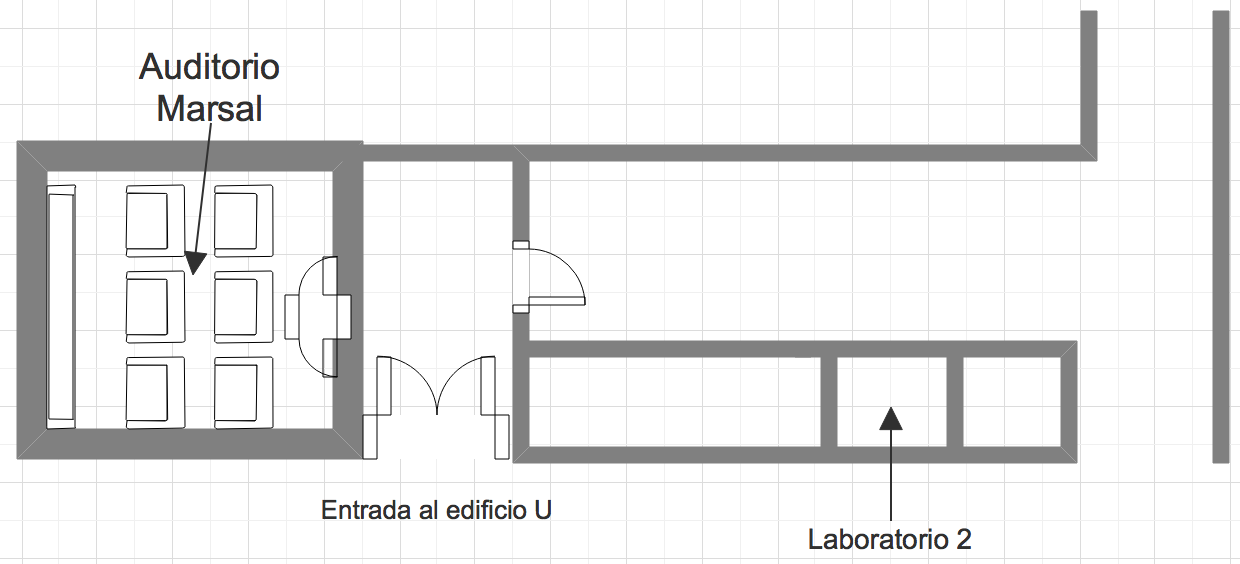
\includegraphics[width=1.0\textwidth]{images/mapa.png}
	\label{mapa}
\end{figure}
\end{frame}

\begin{frame}\frametitle{\rule{0mm}{10mm}\rule{5mm}{0mm} Computación Gráfica. }
\begin{enumerate}
	\item OpenGL 4.0
	\item Visual studio 2017 (Windows) o Eclipse kepler (Ubuntu)
\end{enumerate}
\end{frame}

\begin{frame}\frametitle{\rule{0mm}{10mm}\rule{5mm}{0mm} Evaluación. }
\begin{enumerate}
	\item Previos	20 \%
	\item Practicas 40\%
	\item Proyecto 40 \%	
\end{enumerate}
\end{frame}

\begin{frame}\frametitle{\rule{0mm}{10mm}\rule{5mm}{0mm} Grupo del curso. }
\begin{enumerate}
	\item Inscribirse al grupo: \hfill \break
	https://groups.google.com/d/forum/labcgeihc-2020-1
\end{enumerate}
\end{frame}

\end{document}

